\documentclass[10pt]{article}
\usepackage{ucs}
\usepackage[a4paper, total={6in, 10in}]{geometry}
\usepackage[utf8x]{inputenc}
\usepackage{graphicx}
\title{Essential Skills: Assignment Web services}
\date{2 October 2016}
\author{Ali Abdulmadzhidov}

\begin{document}
\renewcommand*\rmdefault{cmss}
\maketitle
\section{REST calculator}
Caluclator can add,subtract,multiply or divide 2 vars.

Written on python, using Flask framework.
If you try to make GET query on it, it'll answer with message. \\ \\
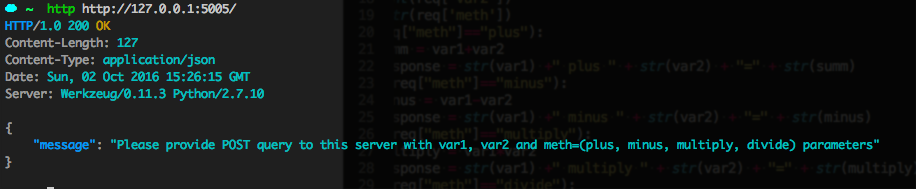
\includegraphics[scale=0.5]{get} \\ \\
You can work with calculater via POST method \\ \\ 
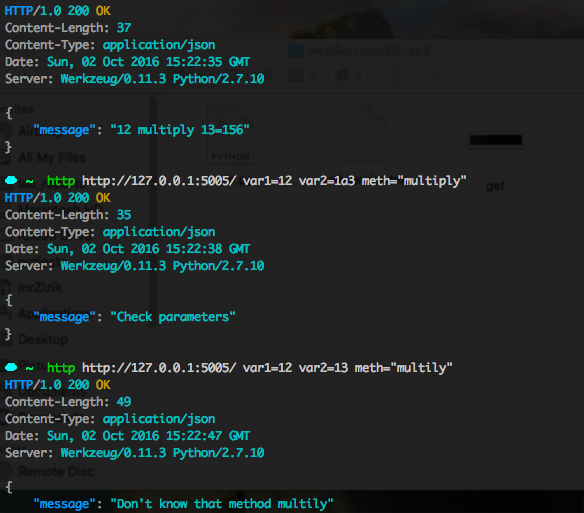
\includegraphics[scale=0.5]{post}


\subsection{Code:}
\begin{verbatim}
#!flask/bin/python
from flask import Flask, jsonify, request

app = Flask(__name__)
from pprint import pprint as pprint
import json

@app.route('/', methods=['GET'])
def hello():
    return jsonify({'message': 'Please provide POST query to this server with var1, var2 and meth=(plus, minus, multiply, divide) parameters'})

@app.route('/', methods=['POST'])
def calc():
    response = ""
    req = json.loads(request.data)
    if checkVars(req):
        var1=int(req['var1'])
        var2=int(req['var2'])
        meth=str(req['meth'])
        if (req["meth"]=="plus"):
            summ = var1+var2
            response = str(var1) +" plus " + str(var2) + "=" + str(summ)
        elif (req["meth"]=="minus"):
            minus = var1-var2
            response = str(var1) +" minus " + str(var2) + "=" + str(minus)
        elif (req["meth"]=="multiply"):
            multiply = var1*var2
            response = str(var1) +" multiply " + str(var2) + "=" + str(multiply)
        elif (req["meth"]=="divide"):
            divide = var1/var2
            response = str(var1) +" divide " + str(var2) + "=" + str(divide)
        else:
            response = "Don't know that method " + meth
    else:
        response = "Check parameters"
    return jsonify({'message': response})

def checkVars(req):
    return req['var1'].isdigit() and req['var2'].isdigit() and req['meth']!= None

if __name__ == '__main__':
    app.run(host='0.0.0.0', port=5005, debug=True)
\end{verbatim}


\end{document}